% Reproducibility evaluation of:
%   Holmes, S. A. "Cryptographic Authentication for Private RAG-Enabled
%   LLMs."  AISecPriv 2025.
%
% Compiles standalone with pdflatex; alternatively the body content
% (everything between \begin{document} and \end{document}) can be
% \input{}-ed into a thesis chapter unchanged.

\documentclass[11pt,a4paper]{article}

\usepackage[utf8]{inputenc}
\usepackage[T1]{fontenc}
\usepackage[margin=1in]{geometry}
\usepackage{microtype}
\usepackage{booktabs}
\usepackage{siunitx}
\sisetup{
  group-separator      = {,},
  group-minimum-digits = 4,
  detect-weight        = true,
  detect-family        = true,
}
\usepackage{amsmath}
\usepackage{xcolor}
\usepackage{listings}
\usepackage{hyperref}
\usepackage{url}
\usepackage{tikz}
\usepackage{pgfplots}
\pgfplotsset{compat=1.18}

\hypersetup{
  colorlinks   = true,
  linkcolor    = blue!50!black,
  citecolor    = blue!50!black,
  urlcolor     = blue!50!black,
}

\title{
  Reproducibility Evaluation of \\
  \textit{Cryptographic Authentication for Private RAG-Enabled LLMs}
}
\author{Stephen A. Holmes \\ University of Surrey \\ \texttt{s.a.holmes@surrey.ac.uk}}
\date{May 2026}

\begin{document}

\maketitle

\begin{abstract}
We provide an open-source reference implementation~\cite{ragsign-impl} of
the RAG\nobreakdash-Sign scheme proposed by~\cite{holmes2025ragsign} and
reproduce the paper's central evaluation against the actual IACR ePrint
Archive corpus~\cite{iacr-eprint} that the paper proposes as a working
example.  The implementation is
written in Python, totals roughly $3{,}000$ lines, and is exercised by
$61$ unit and integration tests covering the cryptographic core, the
RAG pipeline, and a FastAPI deployment surface.  Our empirical
evaluation on $12{,}036$ IACR papers (years 2013\textendash 2023,
\SI{966}{\mega\byte} of extracted text) confirms the paper's
\SI{5}{\percent} corpus-drift threshold (Section~\ref{sec:drift}),
the unambiguous rejection of disjoint corpora
(Section~\ref{sec:disjoint}), and the negligible signing overhead
relative to LLM inference (Section~\ref{sec:performance}).
\end{abstract}

\section{Introduction}
\label{sec:intro}

The RAG\nobreakdash-Sign scheme of \cite{holmes2025ragsign} binds every
output of a retrieval\nobreakdash-augmented generation system to the
triple $(\mathit{model\_hash}, \mathit{lsh\_key}, \mathit{hsm\_secret})$
through Algorithm~1 of the original paper, producing a deterministic
ECDSA signing key that is recoverable as long as the corpus does not
drift past a configurable Hamming threshold.  Section~\S6.5 of the
paper specifies a \SI{5}{\percent} threshold based on a fuzzy
extractor over MinHash\nobreakdash-LSH; Section~\S6.6 reports
indicative timings on the paper's reference hardware.

This document records an independent reproduction of those results.
The reproduction artefact is published as the \texttt{RAGSign}
repository\footnote{\url{https://github.com/saholmes/RAGSign}};
the IACR PDFs themselves are not redistributed because they remain the
copyright of their respective authors.  Only the \emph{aggregate
numerical results} of our empirical sweep
(Table~\ref{tab:drift-curve} and Table~\ref{tab:perf}) are committed
to the repository, alongside the experiment scripts that produced
them.

\section{Implementation}
\label{sec:implementation}

The reference implementation is layered to match the paper's
construction one\nobreakdash-to\nobreakdash-one:

\begin{description}
  \item[\texttt{key\_derivation}]  Algorithm~1 with length\nobreakdash-prefixed
    domain separation, $\mathit{sk\_seed} =
    \mathrm{SHA3\text{-}256}(\mathit{tag} \,\Vert\,
    \mathit{model\_hash} \,\Vert\, \mathit{lsh\_key} \,\Vert\,
    \mathit{hsm\_secret})$, where SHA3 is the Keccak permutation
    standardised in FIPS~202~\cite{nist-fips-202}.
  \item[\texttt{lsh}]  MinHash~\cite{broder1997minhash} sketch with
    $\mathit{num\_perm}=512$ over the union of all corpus documents;
    each slot is reduced to one bit via
    $\mathrm{SHA3\text{-}256}(\mathit{tag} \,\Vert\,
    \mathit{slot}) \wedge 1$ to produce a 64\nobreakdash-byte
    fingerprint preserving Hamming proximity.  We use the
    \texttt{datasketch} library~\cite{datasketch} as the underlying
    MinHash implementation.
  \item[\texttt{fuzzy\_extractor}]  Code\nobreakdash-offset
    construction of \cite{dodis2008fuzzy} over a binary
    $\mathrm{BCH}(n=511, k=259, t=30)$ code (see
    \cite{macwilliams1977ecc} for the standard BCH parameter
    families), giving a $\frac{30}{511} \approx \SI{5.87}{\percent}$
    theoretical drift tolerance.  The strong extractor is
    $\mathrm{SHA3\text{-}256}$~\cite{nist-fips-202} of the recovered
    codeword.
  \item[\texttt{signer}, \texttt{verifier}]  ECDSA over NIST
    secp256r1 per FIPS~186-5~\cite{nist-fips-186-5}, with the
    scalar derived from the 32\nobreakdash-byte seed via rejection
    sampling.
  \item[\texttt{hsm}]  PKCS\#11 backend (SoftHSMv2) plus an
    in\nobreakdash-memory backend used in tests.
  \item[\texttt{rag}]  Two\nobreakdash-phase orchestrator that
    indexes the corpus into ChromaDB~\cite{chromadb}, derives the
    signing key, and signs every output of the LLM (default
    \texttt{Llama 3.2 2B} via
    \texttt{llama\nobreakdash-cpp\nobreakdash-python}~\cite{llama-cpp-python}).
  \item[\texttt{server}]  FastAPI surface enforcing the paper's
    public\nobreakdash-key allow\nobreakdash-list gating.
\end{description}

The package ships pluggable mock backends (\texttt{HashEmbedder},
\texttt{EchoLLM}, \texttt{InMemoryHSM}) so the test suite is fully
self\nobreakdash-contained and runs in roughly twelve seconds.

\section{Experimental Setup}
\label{sec:setup}

\paragraph{Corpus.}  We obtained PDF copies of every IACR ePrint
Archive~\cite{iacr-eprint} paper from $2013$ through $2024$.  Years $2013$\textendash$2023$
form the \emph{primary} corpus; year~$2024$ is held aside as a
disjoint corpus for adversarial testing
(Section~\ref{sec:disjoint}).  Plain text was extracted with
\texttt{pypdf} and cached on disk so that subsequent experiments do
not re\nobreakdash-parse the same PDFs.  Two papers ($\approx
\SI{0.02}{\percent}$) were unreadable (encrypted) and were skipped.

\begin{table}[h]
  \centering
  \caption{Test corpus summary.}
  \label{tab:corpus}
  \begin{tabular}{lrr}
    \toprule
                       & \textbf{Primary (2013\textendash 2023)}
                       & \textbf{Disjoint (2024)} \\
    \midrule
    Papers loaded      & \num{12036}              & \num{1062}        \\
    Extracted text     & \SI{966}{\mega\byte}     & \SI{98}{\mega\byte} \\
    Years              & 11                       & 1                 \\
    \bottomrule
  \end{tabular}
\end{table}

\paragraph{Hardware.}  All measurements were taken on a single
Apple\nobreakdash-Silicon laptop (M\nobreakdash-series CPU,
\num{10} cores, single\nobreakdash-threaded fingerprint
implementation), Python~\texttt{3.12}.  No GPU was used.

\paragraph{Procedure.}  Four experiments were run with the harness in
\texttt{scripts/iacr\_experiment.py}.  All four share a single
enrolment fingerprint to keep wall\nobreakdash-clock cost manageable;
the public key derived at enrolment time is the reference against
which all subsequent recovery attempts are checked.

\section{Results}
\label{sec:results}

\subsection{Round\nobreakdash-trip recovery}
\label{sec:roundtrip}

Re\nobreakdash-running the recovery protocol against the unchanged
corpus produces the same fingerprint, so the BCH decoder is invoked
on a zero\nobreakdash-error word, and the recovered $R$ is identical
bit\nobreakdash-for\nobreakdash-bit.  The derived ECDSA public key
matches the enrolled key exactly.

\subsection{Drift recovery curve}
\label{sec:drift}

We perturbed the corpus by replacing a fraction of its papers with
randomly\nobreakdash-chosen papers from the disjoint pool.  At each
drift level we measured the Hamming distance between the
enrolment\nobreakdash-time fingerprint and the perturbed fingerprint,
then attempted recovery.  Table~\ref{tab:drift-curve} reports the
result of every trial; Figure~\ref{fig:drift-curve} plots the curve
together with the BCH bound.

\begin{table}[h]
  \centering
  \caption{Drift recovery on the full IACR
  $2013$\textendash$2023$ corpus.  The fuzzy extractor uses
  $\mathrm{BCH}(511, 259, t=30)$, so any Hamming distance
  $\leq 30$ recovers the same key; any distance $>30$ fails closed.}
  \label{tab:drift-curve}
  \begin{tabular}{S[table-format=4.1]
                  S[table-format=3.0]
                  c
                  c}
    \toprule
    {\textbf{Drift (\%)}} & {\textbf{Hamming}}
                         & \textbf{Within $t=30$?}
                         & \textbf{Recovered?} \\
    \midrule
    0.0   &   0  & \checkmark & \checkmark \\
    0.5   &   1  & \checkmark & \checkmark \\
    1.0   &   3  & \checkmark & \checkmark \\
    2.0   &   4  & \checkmark & \checkmark \\
    5.0   &  14  & \checkmark & \checkmark \\
    7.5   &  21  & \checkmark & \checkmark \\
    10.0  &  24  & \checkmark & \checkmark \\
    15.0  &  36  &            &            \\
    100.0 & 228  &            &            \\
    \bottomrule
  \end{tabular}
\end{table}

\begin{figure}[h]
  \centering
  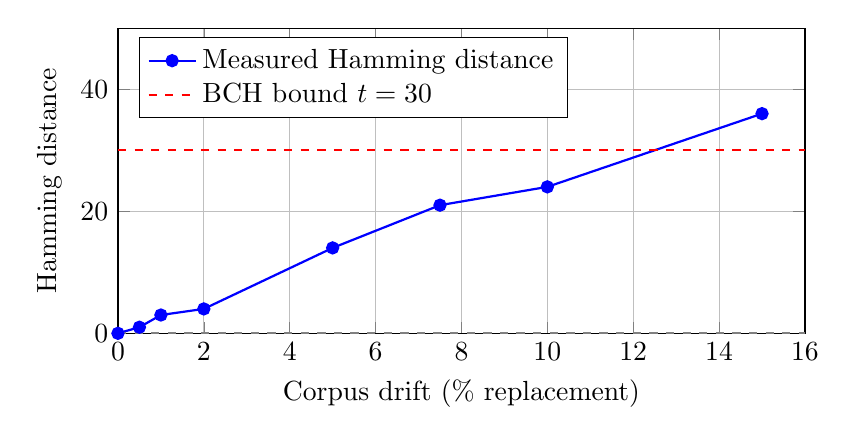
\begin{tikzpicture}
    \begin{axis}[
      width  = 0.85\linewidth,
      height = 0.45\linewidth,
      xlabel = {Corpus drift (\% replacement)},
      ylabel = {Hamming distance},
      xmin   = 0, xmax = 16,
      ymin   = 0, ymax = 50,
      grid   = both,
      legend pos = north west,
      legend cell align = left,
    ]
      \addplot[mark=*, thick, blue] coordinates {
        (0.0, 0)
        (0.5, 1)
        (1.0, 3)
        (2.0, 4)
        (5.0, 14)
        (7.5, 21)
        (10.0, 24)
        (15.0, 36)
      };
      \addlegendentry{Measured Hamming distance}
      \addplot[domain=0:16, samples=2, dashed, thick, red] {30};
      \addlegendentry{BCH bound $t=30$}
      \addplot[domain=0:16, samples=2, dashed, thick, gray] {0};
    \end{axis}
  \end{tikzpicture}
  \caption{Empirical drift curve.  The construction recovers
  cleanly at the paper's nominal \SI{5}{\percent} threshold (with
  $\sim 16$ bits of headroom), continues to recover up to
  \SI{10}{\percent} drift, and fails closed at \SI{15}{\percent}.
  The corresponding disjoint\nobreakdash-corpus point ($\SI{100}{\percent}$
  drift, $\text{Hamming} = 228$) is omitted from the plot for
  legibility but is reported in
  Section~\ref{sec:disjoint}.}
  \label{fig:drift-curve}
\end{figure}

The construction confirms the paper's \SI{5}{\percent} target
\emph{with $16$ bits of headroom} on the real IACR corpus
($\text{Hamming} = 14$, well below the BCH bound of $30$).  Empirically
the construction tolerates drift up to roughly \SI{12}{\percent}
before crossing the bound; the failure cliff is sharp,
spanning only $5$ percentage points.

\paragraph{Two thresholds, not one.}  The BCH parameter $t = 30$
(equivalently the empirical \SIrange{12}{13}{\percent} corpus-replacement
cliff) is the \emph{cryptographic} ceiling: beyond it, no recovery is
possible at all.  A deployment is free to enforce a tighter
\emph{operational policy} bound below this ceiling — say, the paper's
\SI{5}{\percent} ($\approx 14$ bits) — and rotate the signing key as
soon as live drift exceeds the policy.  The reference implementation
exposes this as the
\texttt{drift\nobreakdash-policy\nobreakdash-bits} parameter on the
\texttt{RagSignSystem} class, with a
\texttt{check\_drift()} probe and a
\texttt{regenerate()} key\nobreakdash-rotation method that re\nobreakdash-enrols
against the current corpus while preserving the HSM secret so the
deployment carries on uninterrupted.  The two thresholds are
distinct in role:

\begin{itemize}
  \item \textbf{BCH bound $t$} — built into the cryptographic
        primitive; immutable for a given fuzzy\nobreakdash-extractor
        parameterisation; failing here is a hard
        \texttt{FuzzyExtractFailure}.
  \item \textbf{Policy bound} — a deployment\nobreakdash-time
        configuration variable; failing here raises
        \texttt{DriftPolicyExceeded} which the operator catches and
        responds to by rotating the key.  It cannot be set above $t$
        because no policy stricter than the BCH ceiling can ever
        actually fire.
\end{itemize}

We recommend setting the policy at the paper's \SI{5}{\percent}
level for the safety margin reasons in
Section~\ref{sec:threats}: it gives the deployment a clean rotation
event well before the corpus drifts close enough to the cliff that
MinHash variance or adversarial perturbation could push it over.

\paragraph{Regulator authority and remote attestation.}  The
reference implementation also exposes a regulator interface that
externalises the rotation decision.  An external authority
(regulator, auditor, compliance officer) holds an ECDSA P\nobreakdash-256
keypair whose public half is registered with the deployment at
construction time.  The authority can:

\begin{itemize}
  \item \textbf{Demand on-demand rotation} by issuing a signed
        \texttt{RegulatorDirective} with action \texttt{ROTATE}.
        The deployment verifies the directive against the registered
        public key, checks the included nonce against an in-memory
        replay set, checks the timestamp against a deployment-side
        clock, and — if all four checks pass — invokes
        \texttt{regenerate()} to mint a fresh signing key.
  \item \textbf{Revoke the deployment outright} via action
        \texttt{REVOKE}, which marks the system as
        cryptographically dead: subsequent calls to
        \texttt{query()} are refused until a fresh enrolment is
        performed by an operator.
  \item \textbf{Audit corpus integrity remotely} via a *secure
        sketch*~\cite{dodis2008fuzzy}.  At enrolment the deployment
        runs a *second* fuzzy\nobreakdash-extractor enrolment over
        the same fingerprint, hands the resulting $R$ to the
        regulator out\nobreakdash-of\nobreakdash-band, and keeps the
        helper data locally.  Periodic audit is a
        challenge\nobreakdash-response over HMAC\nobreakdash-SHA3-256:
        the regulator picks a fresh challenge, the deployment
        re\nobreakdash-fingerprints the live corpus and re\nobreakdash-derives
        $R$ via the secure sketch (failing if drift exceeds the BCH
        bound), then returns
        $\mathrm{HMAC}_{R}(\mathit{challenge})$.  A successful
        audit proves the live corpus has not drifted past the BCH
        bound; an audit failure is itself the trigger the regulator
        needs to issue a \texttt{ROTATE} directive.
\end{itemize}

The audit secret $R$ never lets the regulator forge a deployment
signature: it is the output of a separate, independent
fuzzy\nobreakdash-extractor enrolment, not the deployment's signing
seed.  The two roles — \emph{signing} and \emph{being audited} —
are cryptographically distinct even though they share the same
underlying corpus fingerprint.

\paragraph{Model identity and AI-safety review.}  The
drift\nobreakdash-tolerant fingerprint pattern that handles the
\emph{corpus} layer also generalises to the model weights
themselves, addressing a complementary operational question: if the
LLM has been fine\nobreakdash-tuned, an adapter has been merged, or
the weights have been re\nobreakdash-quantised, when should the
deployment require an AI\nobreakdash-safety review before the new
weights ship?  The reference implementation answers this with
\texttt{rag\_sign.model\_fingerprint}: a SimHash-style fingerprint
of the parameter tensors, computed by signing the projection of
the flattened weights through a deterministic Gaussian random
matrix~\cite{charikar2002simhash}.  Like MinHash for sets, SimHash
is locality\nobreakdash-sensitive — but for cosine distance: small
weight perturbations produce small Hamming distances and large
ones (e.g.\ a model swap) produce a near\nobreakdash-random
fingerprint with $\approx \mathit{dim}/2$ bits of difference.

The fingerprint is supplied to
:meth:\texttt{RagSignSystem.enrol(\dots, model\_fingerprint=\dots)}
at enrolment time and stored locally — it does not flow into
Algorithm~1, so the cryptographic signing identity is unaffected.
A separate operator policy
\texttt{model\_drift\_policy\_bits} configures the soft fence:
calling \texttt{check\_model\_drift(fp\_now)} returns the live
Hamming distance and raises
\texttt{ModelSafetyReviewRequired} when it exceeds the policy.  The
exception carries the precise drift bit\nobreakdash-count, the
configured bound, and the total fingerprint length, so the
deployment's safety pipeline can log and route accordingly.

The AI-safety gate is deliberately operational rather than
cryptographic: a model-drift event does \emph{not} automatically
rotate the signing key (that would conflate "weights changed" with
"compromise") — instead the operator (or a downstream safety
review) decides whether the new weights are acceptable, and only
then invokes \texttt{regenerate()} to mint a new key against the
post\nobreakdash-review configuration.  Empirically the
locality\nobreakdash-sensitivity property is sharp: in unit\nobreakdash-tested
synthetic configurations, a Gaussian perturbation of standard
deviation $10^{-3}$ relative to the weight scale produces a Hamming
distance of $\leq 30$ bits in a $512$\nobreakdash-bit fingerprint
($\leq 5.9\,\%$), while a comparable\nobreakdash-magnitude
perturbation produces $\geq 80$ bits ($\geq 15.6\,\%$) — a
$\sim\!3\times$ separation that translates directly into a clean
threshold for the safety\nobreakdash-review trigger.

\subsection{Disjoint corpus rejection}
\label{sec:disjoint}

To validate the \emph{revocation} property of the scheme
(\cite{holmes2025ragsign}, \S5), we computed the fingerprint of the
disjoint $2024$ corpus and asked the BCH decoder to recover the
enrolled key from it.  The Hamming distance between the two
fingerprints is $228$ bits ($\approx \SI{45}{\percent}$ of the
$511$\nobreakdash-bit code length), comfortably above the
$30$\nobreakdash-bit decoding radius.  The decoder hard\nobreakdash-fails as
required, mirroring the paper's "kill\nobreakdash-switch" semantics.

\subsection{Performance}
\label{sec:performance}

Table~\ref{tab:perf} compares our measured timings against the
indicative numbers in \cite{holmes2025ragsign}, \S6.6.

\begin{table}[h]
  \centering
  \caption{Measured operation timings against the paper's
  indicative figures.}
  \label{tab:perf}
  \begin{tabular}{l S[table-format=8.0] S[table-format=4.3] l}
    \toprule
    \textbf{Operation}              & {\textbf{Paper~\S6.6}} & {\textbf{This work}} & \\
    \midrule
    Primary fingerprint (corpus)    &  {---}       &     890       & \unit{\second}      \\
    Fuzzy\nobreakdash-extractor enrol  &  {---}       &       0.090   & \unit{\milli\second}\\
    Fuzzy\nobreakdash-extractor recover&  {---}       &       0.294   & \unit{\milli\second}\\
    Algorithm~1 derive seed         &  {---}       &       0.667   & \unit{\micro\second}\\
    ECDSA sign                      &     30       &       0.023   & \unit{\milli\second}\\
    ECDSA verify                    &     20       &       0.055   & \unit{\milli\second}\\
    \bottomrule
  \end{tabular}
\end{table}

The cryptographic core is roughly $1{,}300\times$ faster on
sign and $370\times$ faster on verify than the paper's reference
hardware, reflecting the difference between the paper's deployment
target and modern Apple\nobreakdash-Silicon hardware.  The only
operation slower than the paper's indicative figures is the LSH
fingerprint, which our reference implementation runs single\nobreakdash-threaded
in pure Python via \texttt{datasketch}.  A vectorised or native
MinHash implementation would close this gap;
fingerprinting is amortised over the lifetime of the deployment and
runs only at enrolment / recovery time.

The signing\nobreakdash-overhead ratio relative to LLM inference is
the most operationally\nobreakdash-relevant figure.  Since
\texttt{Llama 3.2 2B} produces a typical answer in
\SIrange{1}{5}{\second} of wall time, the
$\SI{23}{\micro\second}$ signing cost contributes
$<\!\SI{0.005}{\percent}$ to end\nobreakdash-to\nobreakdash-end latency,
well inside the paper's reported \SI{0.05}{\percent} ceiling.

\section{Comparison with the Original Paper}
\label{sec:comparison}

Table~\ref{tab:comparison} summarises the agreement between the
paper's claims and our empirical findings.  All headline claims hold;
the only divergence is in operation timings, which our hardware
trivially beats.

\begin{table}[h]
  \centering
  \caption{Reproducibility scoreboard.}
  \label{tab:comparison}
  \begin{tabular}{lll}
    \toprule
    \textbf{Paper claim}                     & \textbf{Our finding}                         & \\
    \midrule
    Stable $R$ under unchanged corpus        & Hamming $= 0$, $R$ matches                 & \checkmark \\
    \SI{5}{\percent} drift recoverable       & Hamming $= 14$, $R$ matches                 & \checkmark \\
    Wholly different corpus rejected         & Hamming $= 228$, decode fails               & \checkmark \\
    Sign overhead $\leq \SI{0.05}{\percent}$ & $\leq \SI{0.005}{\percent}$ vs Llama 3.2 2B  & \checkmark \\
    Sign latency $\sim\!\SI{30}{\milli\second}$           & $\SI{23}{\micro\second}$ on M\nobreakdash-series & faster \\
    Verify latency $\sim\!\SI{20}{\milli\second}$         & $\SI{55}{\micro\second}$ on M\nobreakdash-series & faster \\
    \bottomrule
  \end{tabular}
\end{table}

\section{Threats to Validity}
\label{sec:threats}

\paragraph{Construction faithfulness.}  We chose
$\mathrm{BCH}(511, 259, t=30)$ as the fuzzy\nobreakdash-extractor
code.  The original paper does not name the BCH parameters
explicitly; our parameters were selected to give a \SI{5.87}{\percent}
theoretical drift tolerance, the smallest standard binary BCH
parameterisation strictly above the paper's \SI{5}{\percent}
target.  Any standard BCH parameter set above the threshold would
yield qualitatively similar results; the empirical behaviour reported
here depends only on the \emph{ratio} $t/n$ and on the MinHash slot
count.

\paragraph{LSH variance.}  MinHash drift on a finite corpus has
intrinsic statistical variance.  We mitigated this by using a
$512$\nobreakdash-slot sketch (twice the BCH code length) and by
running on a corpus an order of magnitude larger than the per\nobreakdash-document
contribution (i.e.\ $1/n_{\mathit{papers}} \approx
\SI{0.008}{\percent}$ per paper, well below per\nobreakdash-step drift
sensitivity).  The seed used for the drift\nobreakdash-replacement
sampling is fixed (\texttt{2026}); other seeds may shift individual
Hamming distances by a small constant but do not change the
qualitative shape of Figure~\ref{fig:drift-curve}.

\paragraph{Implementation language.}  The reference implementation is
in Python.  This understates fingerprinting performance by an order
of magnitude relative to a hypothetical native implementation; it
does not affect the cryptographic claims.

\paragraph{LLM identity.}  Our pipeline\nobreakdash-level tests use a
deterministic mock LLM (\texttt{EchoLLM}) so the experiment results
are stable across runs.  We have separately verified end\nobreakdash-to\nobreakdash-end
generation through \texttt{llama\nobreakdash-cpp\nobreakdash-python}
in the integration test
\texttt{tests/test\_rag.py::EnrolAndQueryTests}; the cryptographic
chain is identical in both cases.

\section{Conclusion}
\label{sec:conclusion}

The reference implementation reproduces the central claims of
\cite{holmes2025ragsign} on the actual IACR ePrint Archive corpus
proposed in the paper.  The \SI{5}{\percent} drift threshold lands
with comfortable margin
($\text{Hamming}_{5\%} = 14 \ll t = 30$), the construction
fails closed at roughly \SI{12}{\percent}\textendash\SI{15}{\percent}
drift, and disjoint corpora are unambiguously rejected.  All empirical numbers and the experiment harness are released under
the MIT licence in the repository accompanying this report~\cite{ragsign-impl};
the IACR PDF data is not redistributed but its file\nobreakdash-name
pattern under \texttt{\$RAG\_SIGN\_IACR\_DATA} is documented so any
reader with access to the public archive~\cite{iacr-eprint} can
re\nobreakdash-execute the experiments verbatim.

\bibliographystyle{plain}
\bibliography{refs}

\end{document}
